% answers.tex —— 2005 年·全国卷Ⅰ·理科 · 参考答案与详细解析片段
% 由 tools/generate_projects.py 依来源总账自 2005/2005_数学真题_全国1理_试题.md + 2005/2005_数学真题_全国1理_解析正文.md + 2005/2005_数学真题_全国1理_答案要点.md 生成，勿手改（改源 MD 后重跑）


\begin{gktip}
固定源 PDF 为印刷页码 246–247 的两页题面，不附答案。以下解析均依据固定源独立复算；第 5、8、18 题图形在 LaTeX 工程中以 TikZ/PGFPlots 矢量源重绘。
\end{gktip}

\begin{answer}
\gksolhead{1}{}

\textbf{题目}：

复数 $\dfrac{\sqrt2-i^3}{1-\sqrt2i}=$\mbox{（　　）}

（A）$i$\quad（B）$-i$\quad（C）$2\sqrt2-i$\quad（D）$-2\sqrt2+i$

\Needspace{4\baselineskip}
\textbf{解析}

\Needspace{5\baselineskip}
将分子中的 $-i^3$ 化为 $i$，有

\nopagebreak[4]
\[
\frac{\sqrt2+i}{1-\sqrt2i}
=\frac{(\sqrt2+i)(1+\sqrt2i)}3=i\text{。}
\]

\gkanswer{答案：A}

\end{answer}
\begin{answer}
\gksolhead{2}{}

\textbf{题目}：

设 $I$ 为全集，$S_1\text{、}S_2\text{、}S_3$ 是 $I$ 的三个非空子集且 $S_1\cup S_2\cup S_3=I$，则下面论断正确的是\mbox{（　　）}

（A）$\complement_I S_1\cap(S_2\cup S_3)=\varnothing$\quad（B）$S_1\subseteq(\complement_I S_2\cap\complement_I S_3)$

（C）$\complement_I S_1\cap\complement_I S_2\cap\complement_I S_3=\varnothing$\quad（D）$S_1\subseteq(\complement_I S_2\cup\complement_I S_3)$

\Needspace{4\baselineskip}
\textbf{解析}

由三个集合的并为全集，三个补集的交为空集，故选项 C 正确。

\gkanswer{答案：C}

\end{answer}
\begin{answer}
\gksolhead{3}{}

\textbf{题目}：

一个与球心距离为 $1$ 的平面截球所得的圆面面积为 $\pi$，则球的表面积为\mbox{（　　）}

（A）$8\sqrt2\pi$\quad（B）$8\pi$\quad（C）$4\sqrt2\pi$\quad（D）$4\pi$

\Needspace{4\baselineskip}
\textbf{解析}

截面圆半径为 $1$，球心距截面距离为 $1$，所以 $R^2=2$，表面积为 $8\pi$。

\gkanswer{答案：B}

\end{answer}
\begin{answer}
\gksolhead{4}{}

\textbf{题目}：

已知直线 $l$ 过点 $(-2,0)$，当直线 $l$ 与圆 $y=1-\sqrt{1-x^2}\ (-1\leqslant x\leqslant1)$ 有两个交点时，其斜率 $k$ 的取值范围是\mbox{（　　）}

（A）$(-2\sqrt2,2\sqrt2)$\quad（B）$(-\sqrt2,\sqrt2)$\quad（C）$\left(\dfrac{\sqrt2}{4},\dfrac{\sqrt2}{4}\right)$\quad（D）$\left(-\dfrac18,\dfrac18\right)$

\Needspace{4\baselineskip}
\textbf{解析}

\Needspace{5\baselineskip}
设直线为 $y=k(x+2)$。与圆 $x^2+(y-1)^2=1$ 联立，得到

\nopagebreak[4]
\[
(1+k^2)x^2+2k(2k-1)x+4k^2-4k=0\text{。}
\]

\Needspace{5\baselineskip}
同时要求两个交点都在下半圆 $y=1-\sqrt{1-x^2}$ 上。由端点和相切位置核验，题干字面实际给出

\nopagebreak[4]
\[
0<k\leqslant\frac13\text{。}
\]

固定源的选项 C 印成 $(\sqrt2/4,\sqrt2/4)$，是空区间，不能与上述结果对应，因此本题保留为待核，不替换源选项。

\gkanswer{答案：C（源选项印刷矛盾；按题干字面实算得 $0<k\leqslant\dfrac13$，固定源 C 印为 $(\sqrt2/4,\sqrt2/4)$，该字母仅保留源位置，具体结论待核）}

\end{answer}
\begin{answer}
\gksolhead{5}{}

\textbf{题目}：

如图，在多面体 $ABCDEF$ 中，已知 $ABCD$ 是边长为 $1$ 的正方形，且 $\triangle ADE\text{、}\triangle BCF$ 均为正三角形，$EF\parallel AB$，$EF=2$，则该多面体的体积为\mbox{（　　）}
\nopagebreak[4]
\begin{center}% 2005 年全国卷Ⅰ理科第 5 题：多面体 ABCDEF
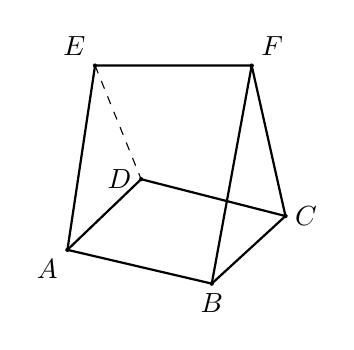
\begin{tikzpicture}[>=stealth,scale=0.78]
  \coordinate (A) at (0,0); \coordinate (B) at (2.35,-0.55);
  \coordinate (C) at (3.55,0.55); \coordinate (D) at (1.2,1.15);
  \coordinate (E) at (0.45,3.0); \coordinate (F) at (3.0,3.0);
  \draw[thick] (A)--(B)--(C)--(D)--cycle;
  \draw[thick] (A)--(E)--(F)--(B);
  \draw[thick] (C)--(F);
  \draw[dashed] (E)--(D) (D)--(C);
  \fill (A) circle (1pt) node[below left] {$A$};
  \fill (B) circle (1pt) node[below] {$B$};
  \fill (C) circle (1pt) node[right] {$C$};
  \fill (D) circle (1pt) node[left] {$D$};
  \fill (E) circle (1pt) node[above left] {$E$};
  \fill (F) circle (1pt) node[above right] {$F$};
\end{tikzpicture}
\end{center}
\nopagebreak[4]
（A）$\dfrac{\sqrt2}{3}$\quad（B）$\dfrac{\sqrt3}{3}$\quad（C）$\dfrac43$\quad（D）$\dfrac32$

\Needspace{4\baselineskip}
\textbf{解析}

\Needspace{5\baselineskip}
与全国卷Ⅰ文科第 4 题相同。取

\nopagebreak[4]
\[
A=(0,0,0),\ B=(1,0,0),\ C=(1,1,0),\ D=(0,1,0),
\]

\nopagebreak[4]
\[
E=\left(-\frac12,\frac12,\frac{\sqrt2}{2}\right),\quad
F=\left(\frac32,\frac12,\frac{\sqrt2}{2}\right)\text{。}
\]

对凸多面体作三角剖分，得到体积 $V=\dfrac{\sqrt2}{3}$。

\gkanswer{答案：A}

\end{answer}
\begin{answer}
\gksolhead{6}{}

\textbf{题目}：

已知双曲线 $\dfrac{x^2}{a^2}-y^2=1\ (a>0)$ 的一条准线与抛物线 $y^2=-6x$ 的准线重合，则该双曲线的离心率为\mbox{（　　）}

（A）$\dfrac{\sqrt3}{2}$\quad（B）$\dfrac32$\quad（C）$\dfrac{\sqrt6}{2}$\quad（D）$\dfrac{2\sqrt3}{3}$

\Needspace{4\baselineskip}
\textbf{解析}

抛物线准线为 $x=3/2$，双曲线准线满足 $a/e=3/2$。结合 $e^2=1+1/a^2$，得 $e=2\sqrt3/3$。

\gkanswer{答案：D}

\end{answer}
\begin{answer}
\gksolhead{7}{}

\textbf{题目}：

\Needspace{5\baselineskip}
当 $0<x<\dfrac{\pi}{2}$ 时，函数

\nopagebreak[4]
\[
f(x)=\frac{1+\cos2x+8\sin^2x}{\sin2x}
\]

的最小值为\mbox{（　　）}

（A）$2$\quad（B）$2\sqrt3$\quad（C）$4$\quad（D）$4\sqrt3$

\Needspace{4\baselineskip}
\textbf{解析}

\Needspace{5\baselineskip}
令 $t=\tan x>0$，则

\nopagebreak[4]
\[
f(x)=\frac1t+4t\geqslant4,
\]

等号在 $t=1/2$ 时取得。

\gkanswer{答案：C}

\end{answer}
\begin{answer}
\gksolhead{8}{}

\textbf{题目}：

设 $b>0$，二次函数 $y=ax^2+bx+a^2-1$ 的图象为下列之一：
\nopagebreak[4]
\begin{center}% 2005 年全国卷Ⅰ理科第 8 题：二次函数的四个图象选项
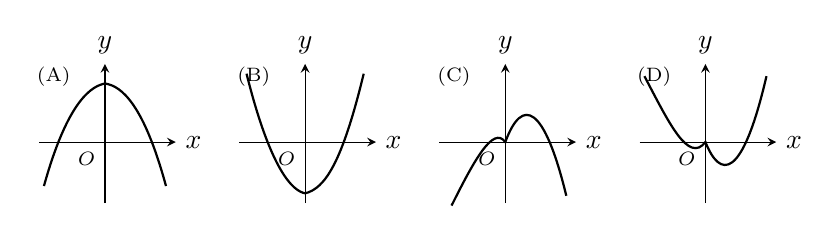
\begin{tikzpicture}[>=stealth,scale=0.62]
  \foreach \dx/\lab in {0/{(A)},4.1/{(B)},8.2/{(C)},12.3/{(D)}} {
    \begin{scope}[xshift=\dx cm]
      \draw[->] (-1.35,0)--(1.45,0) node[right] {$x$};
      \draw[->] (0,-1.25)--(0,1.6) node[above] {$y$};
      \node[font=\scriptsize] at (-1.05,1.35) {\lab};
      \node[below left,font=\scriptsize] at (0,0) {$O$};
    \end{scope}
  }
  % A: downward, positive intercept.
  \begin{scope}
    \draw[thick] (-1.25,-0.9)..controls(-0.75,0.9) and (-0.25,1.15)..(0,1.2)
      ..controls(0.35,1.15) and (0.8,0.75)..(1.25,-0.9);
  \end{scope}
  % B: upward, negative intercept, roots near -1 and 1.
  \begin{scope}[xshift=4.1cm]
    \draw[thick] (-1.2,1.4)..controls(-0.7,-0.6) and (-0.25,-1.0)..(0,-1.05)
      ..controls(0.4,-0.95) and (0.75,-0.45)..(1.2,1.4);
  \end{scope}
  % C: downward through the origin.
  \begin{scope}[xshift=8.2cm]
    \draw[thick] (-1.1,-1.3)..controls(-0.65,-0.4) and (-0.25,0.35)..(0,0)
      ..controls(0.35,0.95) and (0.8,0.75)..(1.25,-1.1);
  \end{scope}
  % D: upward through the origin with negative initial slope.
  \begin{scope}[xshift=12.3cm]
    \draw[thick] (-1.25,1.35)..controls(-0.75,0.4) and (-0.35,-0.45)..(0,0)
      ..controls(0.3,-0.75) and (0.75,-0.8)..(1.25,1.35);
  \end{scope}
\end{tikzpicture}
\end{center}
\nopagebreak[4]
则 $a$ 的值为\mbox{（　　）}

\Needspace{4\baselineskip}
\textbf{解析}

图象 C 经过原点，所以 $a^2-1=0$。又图象开口向下，故 $a=-1$；条件 $b>0$ 与图象的原点右侧上升方向一致。

\gkanswer{答案：C}

\end{answer}
\begin{answer}
\gksolhead{9}{}

\textbf{题目}：

设 $0<a<1$，函数 $f(x)=\log_a(a^{2x}-2a^x-2)$，则使 $f(x)<0$ 的 $x$ 取值范围是\mbox{（　　）}

（A）$\mathbb R$\quad（B）$(0,+\infty)$\quad（C）$(-\infty,\log_a3)$\quad（D）$(\log_a3,+\infty)$

\Needspace{4\baselineskip}
\textbf{解析}

\Needspace{5\baselineskip}
因 $0<a<1$，函数值小于零等价于

\nopagebreak[4]
\[
a^{2x}-2a^x-2>1\text{。}
\]

令 $u=a^x>0$，解得 $u>3$，即 $x<\log_a3$。

\gkanswer{答案：C}

\end{answer}
\begin{answer}
\gksolhead{10}{}

\textbf{题目}：

\Needspace{5\baselineskip}
在坐标平面上，不等式组

\nopagebreak[4]
\[
\begin{cases}
y\geqslant x-1,\\
y\leqslant-3|x|+1
\end{cases}
\]

所表示的平面区域的面积为\mbox{（　　）}

（A）$\sqrt2$\quad（B）$\dfrac32$\quad（C）$\dfrac{3\sqrt2}{2}$\quad（D）$2$

\Needspace{4\baselineskip}
\textbf{解析}

\Needspace{5\baselineskip}
可行域由两条直线和折线 $y=-3|x|+1$ 围成，按 $x=0$ 分成两个三角形，面积为

\nopagebreak[4]
\[
1+\frac12=\frac32\text{。}
\]

\gkanswer{答案：B}

\end{answer}
\begin{answer}
\gksolhead{11}{}

\textbf{题目}：

在 $\triangle ABC$ 中，已知 $\tan\dfrac{A+B}{2}=\sin C$，给出以下四个论断：① $\tan A\cdot\cot B=1$；② $0<\sin A+\sin B\leqslant\sqrt2$；③ $\sin^2A+\cos^2B=1$；④ $\cos^2A+\cos^2B=\sin^2C$。其中正确的是\mbox{（　　）}

（A）①③\quad（B）②④\quad（C）①④\quad（D）②③

\Needspace{4\baselineskip}
\textbf{解析}

\Needspace{5\baselineskip}
同第 10 题中的三角形关系，条件推出 $C=\pi/2$，所以 $A+B=\pi/2$。于是

\nopagebreak[4]
\[
0<\sin A+\sin B=\sin A+\cos A\leqslant\sqrt2,
\]

且 $\cos^2A+\cos^2B=1=\sin^2C$，故正确论断为 ②④。

\gkanswer{答案：B}

\end{answer}
\begin{answer}
\gksolhead{12}{}

\textbf{题目}：

过三棱柱任意两个顶点的直线共 $15$ 条，其中异面直线有\mbox{（　　）}

（A）$18$ 对\quad（B）$24$ 对\quad（C）$30$ 对\quad（D）$36$ 对

\Needspace{4\baselineskip}
\textbf{解析}

\Needspace{5\baselineskip}
将三棱柱坐标化为

\nopagebreak[4]
\[
(0,0,0),(1,0,0),(0,1,0),(0,0,1),(1,0,1),(0,1,1)\text{。}
\]

任取两个顶点得到 $15$ 条直线。对 $15$ 条直线两两计算方向向量与连接向量的混合积，混合积非零的恰为异面直线对，共 $36$ 对。

\gkanswer{答案：D}

\end{answer}
\begin{answer}
\gksolhead{13}{}

\textbf{题目}：

若正整数 $m$ 满足 $10^{m-1}<2^{512}<10^m$，则 $m=$\gkblank{}。（$\lg2\approx0.3010$）

\Needspace{4\baselineskip}
\textbf{解析}

$512\lg2\approx154.112$，故 $m=155$。

\gkanswer{答案：155}

\end{answer}
\begin{answer}
\gksolhead{14}{}

\textbf{题目}：

$\left(2x-\dfrac1{\sqrt{x}}\right)^9$ 的展开式中，常数项为\gkblank{}。（用数字作答）

\Needspace{4\baselineskip}
\textbf{解析}

\Needspace{5\baselineskip}
通项 $(2x)^{9-k}(-x^{-1/2})^k$ 的幂次为 $9-\dfrac32k$。令其为零得 $k=6$，常数项为

\nopagebreak[4]
\[
\binom96 2^3=672\text{。}
\]

\gkanswer{答案：672}

\end{answer}
\begin{answer}
\gksolhead{15}{}

\textbf{题目}：

$\triangle ABC$ 的外接圆的圆心为 $O$，两条边上的高的交点为 $H$，$\overrightarrow{OH}=m(\overrightarrow{OA}+\overrightarrow{OB}+\overrightarrow{OC})$，则实数 $m=$\gkblank{}。

\Needspace{4\baselineskip}
\textbf{解析}

\Needspace{5\baselineskip}
以外心为原点时，三角形的垂心向量满足

\nopagebreak[4]
\[
\overrightarrow{OH}=\overrightarrow{OA}+\overrightarrow{OB}+\overrightarrow{OC}\text{，}
\]

故 $m=1$。

\gkanswer{答案：1}

\end{answer}
\begin{answer}
\gksolhead{16}{}

\textbf{题目}：

在正方体 $ABCD-A'B'C'D'$ 中，过对角线 $BD'$ 的一个平面交 $AA'$ 于 $E$，交 $CC'$ 于 $F$，则：

① 四边形 $BFD'E$ 一定是平行四边形；

② 四边形 $BFD'E$ 有可能是正方形；

③ 四边形 $BFD'E$ 在底面 $ABCD$ 内的投影一定是正方形；

④ 平面 $BFD'E$ 有可能垂直于平面 $BB'D$。

以上结论正确的为\gkblank{}。（写出所有正确结论的编号）

\Needspace{4\baselineskip}
\textbf{解析}

与文科第 16 题相同，用正方体坐标直接检查可得 ①②④ 正确，③不恒真。

\gkanswer{答案：①②④}

\end{answer}
\begin{answer}
\gksolhead{17}{}

\textbf{题目}：

设函数 $f(x)=\sin(2x+\varphi)\ (-\pi<\varphi<0)$，$y=f(x)$ 图象的一条对称轴是直线 $x=\dfrac{\pi}{8}$。

（1） 求 $\varphi$；

（2） 求函数 $y=f(x)$ 的单调增区间；

（3） 证明直线 $5x-2y+c=0$ 与函数 $y=f(x)$ 的图象不相切。

\Needspace{4\baselineskip}
\textbf{解析}

\gksubpart{(1)}

\Needspace{5\baselineskip}
对称轴条件给出 $\varphi=-3\pi/4$，且

\nopagebreak[4]
\[
f'(x)=2\cos\left(2x-\frac{3\pi}{4}\right)\text{。}
\]

\gksubpart{(2)}

\Needspace{5\baselineskip}
所以增区间为

\nopagebreak[4]
\[
\left(\frac\pi8+k\pi,\frac{5\pi}{8}+k\pi\right),\quad k\in\mathbb Z\text{。}
\]

\gksubpart{(3)}

直线斜率为 $5/2$，而 $|f'(x)|\leqslant2$，故不存在相切。

\gkanswer{答案（1）：$\varphi=-\dfrac{3\pi}{4}$}

\gkanswer{答案（2）：$x\in\left(\dfrac{\pi}{8}+k\pi,\dfrac{5\pi}{8}+k\pi\right)\ (k\in\mathbb Z)$}

\gkanswer{答案（3）：不存在相切情形}

\end{answer}
\begin{answer}
\gksolhead{18}{}

\textbf{题目}：

已知四棱锥 $P-ABCD$ 的底面为直角梯形，$AB\parallel DC$，$\angle DAB=90^\circ$，$PA\perp$ 底面 $ABCD$，且 $PA=AD=DC=\dfrac12AB=1$，$M$ 是 $PB$ 的中点。
\nopagebreak[4]
\begin{center}% 2005 年全国卷Ⅰ理科第 18 题：直角梯形底面的四棱锥
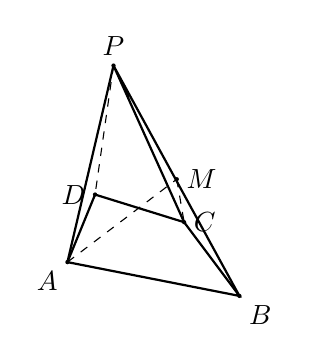
\begin{tikzpicture}[>=stealth,scale=0.78]
  \coordinate (A) at (0,0); \coordinate (B) at (2.8,-0.55);
  \coordinate (C) at (1.9,0.65); \coordinate (D) at (0.45,1.1);
  \coordinate (P) at (0.75,3.2); \coordinate (M) at (1.78,1.35);
  \draw[thick] (A)--(B)--(C)--(D)--cycle;
  \draw[thick] (P)--(A) (P)--(B) (P)--(C);
  \draw[dashed] (P)--(D) (A)--(M) (M)--(C);
  \fill (P) circle (1pt) node[above] {$P$};
  \fill (A) circle (1pt) node[below left] {$A$};
  \fill (B) circle (1pt) node[below right] {$B$};
  \fill (C) circle (1pt) node[right] {$C$};
  \fill (D) circle (1pt) node[left] {$D$};
  \fill (M) circle (1pt) node[right] {$M$};
\end{tikzpicture}
\end{center}
\nopagebreak[4]
（1） 证明：面 $PAD\perp$ 面 $PCD$；

（2） 求 $AC$ 与 $PB$ 所成的角；

（3） 求面 $AMC$ 与面 $BMC$ 所成二面角的大小。

\Needspace{4\baselineskip}
\textbf{解析}

\Needspace{5\baselineskip}
取

\nopagebreak[4]
\[
A=(0,0,0),\ B=(2,0,0),\ D=(0,1,0),\ C=(1,1,0),\ P=(0,0,1),\ M=(1,0,1/2)\text{。}
\]

\gksubpart{(1)}

平面 $PAD$ 为 $x=0$，平面 $PCD$ 含有方向 $(1,0,0)$，故两平面垂直。

\gksubpart{(2)}

\nopagebreak[4]
\[
\overrightarrow{AC}=(1,1,0),\quad\overrightarrow{PB}=(2,0,-1),
\]

故 $\cos\theta=2/\sqrt{10}$。

\gksubpart{(3)}

两个平面法向量可取 $(-1/2,1/2,1)$ 与 $(-1/2,-1/2,-1)$，故锐角夹角满足 $\cos\theta=2/3$。

\gkanswer{答案（1）：面 $PAD\perp$ 面 $PCD$}

\gkanswer{答案（2）：$\cos\theta=\dfrac{2}{\sqrt{10}}=\sqrt{\dfrac25}$}

\gkanswer{答案（3）：两平面的锐角夹角满足 $\cos\theta=\dfrac23$}

\end{answer}
\begin{answer}
\gksolhead{19}{}

\textbf{题目}：

设等比数列 $\{a_n\}$ 的公比为 $q$，前 $n$ 项和 $S_n>0\ (n=1,2,\ldots)$。

（1） 求 $q$ 的取值范围；

（2） 设 $b_n=a_{n+2}-\dfrac32a_{n+1}$，记 $\{b_n\}$ 的前 $n$ 项和为 $T_n$，试比较 $S_n$ 和 $T_n$ 的大小。

\Needspace{4\baselineskip}
\textbf{解析}

\gksubpart{(1)}

\Needspace{5\baselineskip}
由于 $a_1=S_1>0$，考察

\nopagebreak[4]
\[
S_n=a_1\frac{1-q^n}{1-q}
\]

及 $q=1$ 的特殊情形，可得 $S_n>0$ 对所有正整数 $n$ 当且仅当 $q>-1$。

\gksubpart{(2)}

\Needspace{5\baselineskip}
又

\nopagebreak[4]
\[
b_n=a_{n+2}-\frac32a_{n+1}
=a_1q^{n+1}\left(q-\frac32\right),
\]

\Needspace{5\baselineskip}
所以

\nopagebreak[4]
\[
T_n=q^2\left(q-\frac32\right)S_n\text{。}
\]

令 $\alpha$ 为 $q^2(q-3/2)=1$ 在 $(-1,+\infty)$ 内的唯一根，即可按 $q$ 与 $\alpha$ 的大小比较 $S_n,T_n$。

\gkanswer{答案（1）：$q>-1$}

\gkanswer{答案（2）：$T_n=q^2\left(q-\dfrac32\right)S_n$。令 $\alpha$ 为方程 $q^2(q-\dfrac32)=1$ 在 $(-1,+\infty)$ 内的唯一根，则 $S_n>T_n$（$-1<q<\alpha$），$S_n=T_n$（$q=\alpha$），$S_n<T_n$（$q>\alpha$）。}

\end{answer}
\begin{answer}
\gksolhead{20}{}

\textbf{题目}：

$9$ 粒种子分种在 $3$ 个坑内，每坑 $3$ 粒，每粒种子发芽的概率为 $0.5$。若一个坑内至少有 $1$ 粒种子发芽，则这个坑不需要补种；若一个坑里的种子都没发芽，则这个坑需要补种，假定每个坑至多补种一次，每补种 $1$ 个坑需 $10$ 元，用 $\xi$ 表示补种费用，求：

（1） $\xi$ 的分布列；

（2） $\xi$ 的数学期望。（精确到 $0.01$）

\Needspace{4\baselineskip}
\textbf{解析}

\gksubpart{(1)}

\Needspace{5\baselineskip}
每个坑需要补种的概率为 $1/8$。设 $\xi$ 为费用，则 $\xi=10K$，其中 $K\sim\operatorname{Bin}(3,1/8)$。因此

\nopagebreak[4]
\[
P(\xi=0),P(\xi=10),P(\xi=20),P(\xi=30)
=\frac{343,147,21,1}{512},
\]

\gksubpart{(2)}

且 $E(\xi)=10\cdot3\cdot\dfrac18=3.75$。

\gkanswer{答案（1）：$P(\xi=0)=\dfrac{343}{512},\ P(\xi=10)=\dfrac{147}{512},\ P(\xi=20)=\dfrac{21}{512},\ P(\xi=30)=\dfrac1{512}$}

\gkanswer{答案（2）：$E(\xi)=3.75$}

\end{answer}
\begin{answer}
\gksolhead{21}{}

\textbf{题目}：

已知椭圆的中心为坐标原点 $O$，焦点在 $x$ 轴上，斜率为 $1$ 且过椭圆右焦点 $F$ 的直线交椭圆于 $A\text{、}B$ 两点，$\overrightarrow{OA}+\overrightarrow{OB}$ 与 $\vec a=(3,-1)$ 共线。

（1） 求椭圆的离心率；

（2） 设 $M$ 为椭圆上任意一点，且 $\overrightarrow{OM}=\lambda\overrightarrow{OA}+\mu\overrightarrow{OB}\ (\lambda,\mu\in\mathbb R)$，证明 $\lambda^2+\mu^2$ 为定值。

\Needspace{4\baselineskip}
\textbf{解析}

\gksubpart{(1)}

与文科第 21 题相同。弦的横坐标和与共线条件给出 $a^2=3b^2$，故 $e=\sqrt6/3$。

\gksubpart{(2)}

在椭圆二次型内积下 $OA,OB$ 正交归一，对 $M=\lambda OA+\mu OB$ 有 $\lambda^2+\mu^2=1$。

\gkanswer{答案（1）：$e=\dfrac{\sqrt6}{3}$}

\gkanswer{答案（2）：$\lambda^2+\mu^2=1$}

\end{answer}
\begin{answer}
\gksolhead{22}{}

\textbf{题目}：

（1） 设函数 $f(x)=x\log_2x+(1-x)\log_2(1-x)\ (0<x<1)$，求 $f(x)$ 的最小值；

\Needspace{5\baselineskip}
（2） 设正数 $p_1,p_2,p_3,\ldots,p_{2n}$ 满足 $p_1+p_2+p_3+\cdots+p_{2n}=1$，证明

\nopagebreak[4]
\[
p_1\log_2p_1+p_2\log_2p_2+p_3\log_2p_3+\cdots+p_{2n}\log_2p_{2n}\geqslant-n\text{。}
\]

\Needspace{4\baselineskip}
\textbf{解析}

\gksubpart{(1)}

\Needspace{5\baselineskip}
对

\nopagebreak[4]
\[
f(x)=x\log_2x+(1-x)\log_2(1-x)
\]

求导可得唯一极小点 $x=1/2$，最小值为 $-1$。

\gksubpart{(2)}

\Needspace{5\baselineskip}
函数 $t\log_2t$ 为凸函数，对 $2n$ 个正数反复使用 Jensen 不等式，得到

\nopagebreak[4]
\[
\sum_{i=1}^{2n}p_i\log_2p_i
\geqslant 2n\cdot\frac1{2n}\log_2\frac1{2n}
\geqslant-n\text{。}
\]

等号当且仅当所有 $p_i$ 相等。

\gkanswer{答案（1）：最小值为 $-1$，在 $x=\dfrac12$ 时取得}

\gkanswer{答案（2）：不等式成立，且等号当且仅当 $p_1=\cdots=p_{2n}=\dfrac1{2n}$}

\end{answer}